\documentclass[tikz,border=2pt]{standalone}
\usepackage{amsmath,amssymb}
\usepackage{pgfplots}
\pgfplotsset{compat=1.18}

\begin{document}
% Rayleigh density (sigma = 1): the length of a vector whose two coordinates are independent
% N(0, sigma^2); it starts at 0, peaks at x = sigma and has a long right tail.
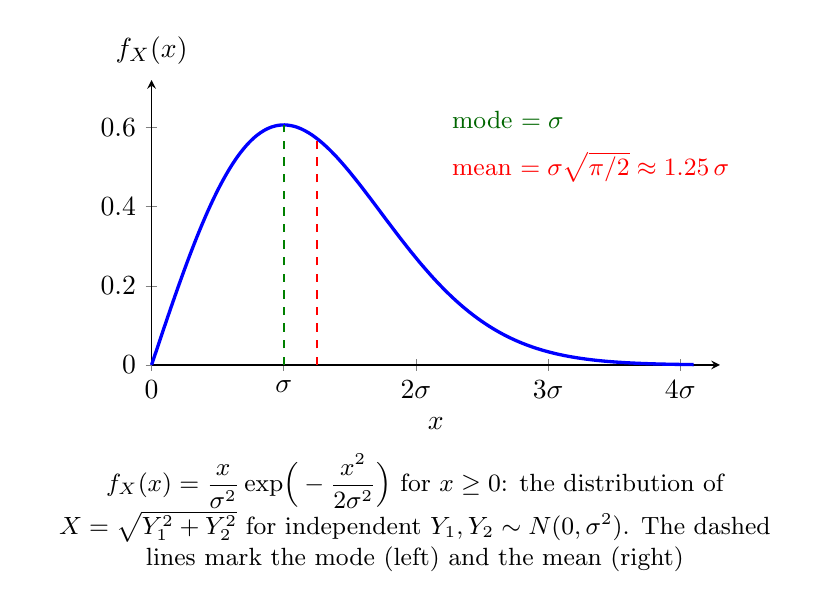
\begin{tikzpicture}
	\begin{axis}[
		axis lines=left, xmin=0, xmax=4.3, ymin=0, ymax=0.72,
		xtick={0,1,2,3,4}, xticklabels={$0$,$\sigma$,$2\sigma$,$3\sigma$,$4\sigma$}, ytick={0,0.2,0.4,0.6},
		xlabel={$x$}, ylabel={$f_X(x)$}, ylabel style={rotate=-90, anchor=south, at={(axis description cs:0,1.02)}},
		samples=160, smooth, width=8.8cm, height=5.2cm, clip=false
		]
		\addplot[blue, very thick, domain=0:4.1] {x*exp(-x^2/2)};
		\draw[green!50!black, dashed, thick] (axis cs:1,0) -- (axis cs:1,0.6065);
		\draw[red, dashed, thick] (axis cs:1.2533,0) -- (axis cs:1.2533,0.571);
		\node[green!40!black, anchor=west, font=\small] at (axis cs:2.2,0.62) {mode $=\sigma$};
		\node[red, anchor=west, font=\small] at (axis cs:2.2,0.5) {mean $=\sigma\sqrt{\pi/2}\approx1.25\,\sigma$};
	\end{axis}
	\node[anchor=north, font=\small, align=flush center, text width=9.6cm] at ([yshift=-2pt]current axis.outer south) {$f_X(x)=\dfrac x{\sigma^2}\exp\!\Big(-\dfrac{x^2}{2\sigma^2}\Big)$ for $x\ge0$: the distribution of $X=\sqrt{Y_1^2+Y_2^2}$ for independent $Y_1,Y_2\sim N(0,\sigma^2)$. The dashed lines mark the mode (left) and the mean (right)};
\end{tikzpicture}
\end{document}
